\section{Obrázky součástek a stavebnic}
\subsection{Renderování součástek}
Jak již bylo zmíněno v~sekci \emph{\ref{reserse-vykresleni}}, Rebrickable poskytuje většinu obrázků vyrenderovaných součástek z~knihovny LDraw volně ke stažení. Pro zbytek součástek jsem implementoval mechanizmus vykreslení s~využitím programů stl2pov \autocite{stl2pov} a POV-Ray \autocite{povray}.

Vykreslení součástek zajišťuje třída \textit{STLRenderer}. Třída nejprve připraví kompletní scénu, obsahující součástku převedenou pomocí stl2pov do POV-Ray formátu. Dále scéna obsahuje definici pozice světel a kamery, specifikované v~souboru \textit{app/Resources/povray\_layout/layout.tmpl}. Následně je pomocí volání programu POV-Ray vykreslen obrázek. 

Porovnání vyrenderované součástky s~obrázkem součástky z~Rebrickable je možné vidět na obrázku \emph{\ref{porovnani-render}}.

\begin{figure}[htbp]
    \centering
    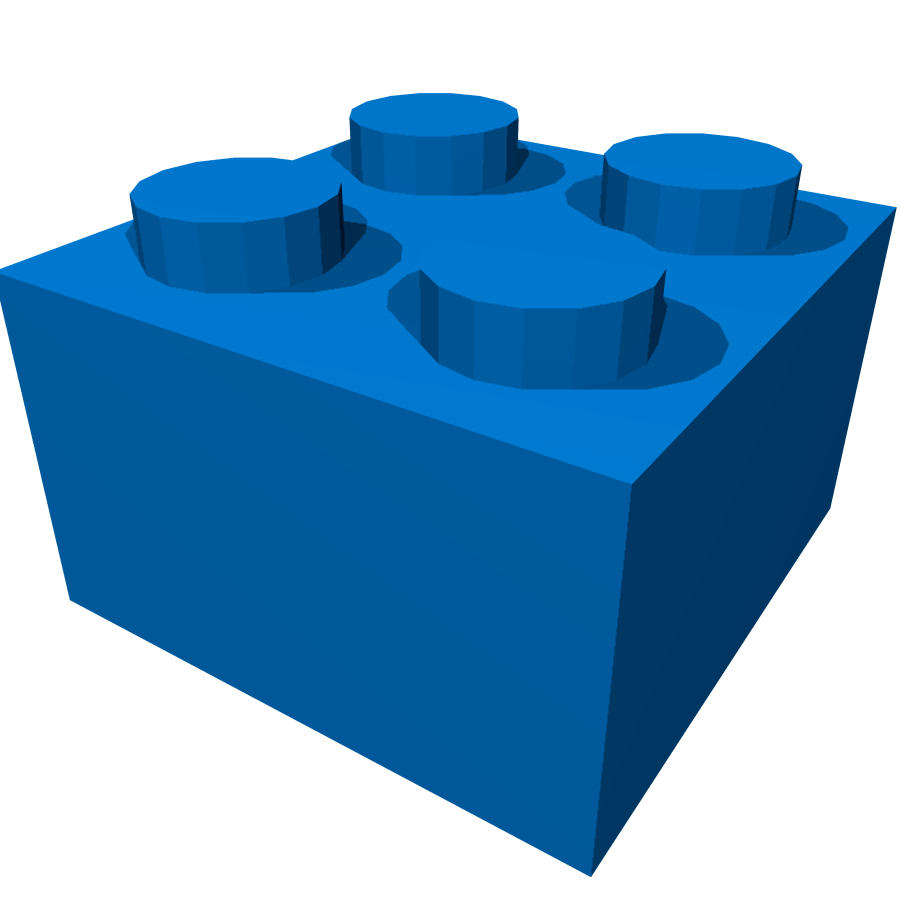
\includegraphics[width=0.30\textwidth,height=\textheight,keepaspectratio]{images/povray.png}
    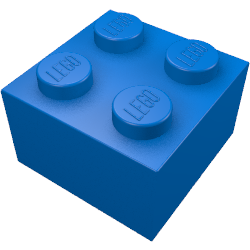
\includegraphics[width=0.30\textwidth,height=\textheight,keepaspectratio]{images/3003.png}
    \caption{Porovnání renderu součástky a Rebrickable \autocite{rebrickable:part:image:3003}\label{porovnani-render}}
\end{figure}


\subsection{Cachování obrázků}
Pro urychlení načítaní webových stránek jsem implementoval mechanizmus cachování miniatur obrázků součástek a stavebnic. K~práci s~obrázky v~Symfony slouží komponenta LiipImagineBundle \autocite{liipimagine}. LiipImagineBundle umožňuje definování různých filtrů a transformací, které jsou aplikovány na zobrazované obrázky. Transformované obrázky jsou následně uloženy do cache, ze které jsou při dalším požadavku načtené.

Proces vytváření transformovaných obrázků se skládá ze tří kroků:
\begin{enumerate}
    \item načtení obrázku,
    \item aplikace flitrů,
    \item uložení transformovaného obrázku do cache.
\end{enumerate}

\subsubsection*{Načtení obrázku}
Načítání obrázků mají na starosti třídy \textit{PartImageLoader} a \textit{SetImageLoader}, které implementují rozhraní \textit{LoaderInterface} a na základě vstupu vrací binární obsah obrázku. 

% \subsubsection*{PartImageLoader}
% Třída \textit{PartImageLoader} má na starost vyhledávání obrázku součástek na základě zadané cesty. 


% \subsubsection*{SetImageLoader}


% http://rebrickable.com/media/parts/ldraw/1/3003.png

\subsubsection*{Aplikace filtrů}
Filtry jsou na obrázky aplikovány na základě konfigurace (ukázka kódu \emph{\ref{liip-imagine-config}}).  

\begin{listing}[htbp]
  \begin{minted}{yaml}
liip_imagine:
    filter_sets:
        part_min:
            quality: 90
            data_loader: part_image_loader
            cache: ~
            default_image: "/resources/images/noimage_min.png"
            filters:
                upscale: { min: [230, 230] }
                thumbnail: { size: [230, 230], mode: inset, allow_upscale: true }
                background: { size: [250, 250], position: center, color: '#FFFFFF' }
  \end{minted}
  \caption{Ukázka konfigurace filtru LiipImagineBundle\label{liip-imagine-config}}
\end{listing}



% \begin{listing}[htbp]
%   \begin{minted}{html}
% <img src="{{ 1/3003.png | imagine_filter(part_min) }}" >
%     \end{minted}
%   \caption{Ukázka použití filtru LiipImagineBundle\label{liip-imagine-usage}}
% \end{listing}   
